\documentclass{article}
\usepackage[UTF8]{ctex}
\usepackage{geometry}
\usepackage{natbib}
\geometry{left=3.18cm,right=3.18cm,top=2.54cm,bottom=2.54cm}
\usepackage{graphicx}
\pagestyle{plain}	
\usepackage{setspace}
\usepackage{caption2}
\usepackage{datetime} %日期
\renewcommand{\today}{\number\year 年 \number\month 月 \number\day 日}
\renewcommand{\captionlabelfont}{\small}
\renewcommand{\captionfont}{\small}
\begin{document}

\begin{figure}
    \centering
    
\includegraphics[width=8cm]{upc.png}

    \label{figupc}
\end{figure}

	\begin{center}
		\quad \\
		\quad \\
		\heiti \fontsize{45}{17} \quad \quad \quad 
		\vskip 1.5cm
		\heiti \zihao{2} 《计算科学导论》课程总结报告
	\end{center}
	\vskip 2.0cm
		
	\begin{quotation}
% 	\begin{center}
		\doublespacing
		
        \zihao{4}\par\setlength\parindent{7em}
		\quad 

		学生姓名:\underline{\qquad  李保辉 \qquad \qquad}

		学\hspace{0.61cm} 号:\underline{\qquad 1907010120\qquad}
		
		专业班级:\underline{\qquad 计科1901 \qquad  }
		
        学\hspace{0.61cm} 院:\underline{计算机科学与技术学院}
% 	\end{center}
		\vskip 2cm
		\centering
		\begin{table}[h]
            \centering 
            \zihao{4}
            \begin{tabular}{|c|c|c|c|c|c|c|}
            % 这里的rl 与表格对应可以看到,姓名是r,右对齐的;学号是l,左对齐的;若想居中,使用c关键字。
                \hline
                课程认识 & 问题思 考 & 格式规范  & IT工具  & Latex附加  & 总分 & 评阅教师 \\
                30\% & 30\% & 20\% & 20\% & 10\% &  &  \\
                \hline
                 & & & & & &\\
                & & & & & &\\
                \hline
            \end{tabular}
        \end{table}
		\vskip 2cm
		\today
	\end{quotation}

\thispagestyle{empty}
\newpage
\setcounter{page}{1}
% 在这之前是封面,在这之后是正文
\section{引言}
    在我上大学之前我对于计算机的知识十分有限。但是,当我到达大学后我才知道了计算机没有我想的没那么简单。尤其是当我上了《计算机导论》这门课程后,我才发现我之前对于计算机的认识是多么的愚蠢。同样也是这门课使我了解了跟多关于计算机的知识,并且我对我自己的专业有了更加清楚的认识。

    我第一次听说鸿蒙操作系统是在中美贸易战的时候听到的。当时,我就对他产生了兴趣。当我看到了我们选的课题中有这个课题时我毫不犹豫的和我的搭档商量。幸运的是我的搭档也和我一样对鸿蒙操作系统感兴趣。于是,我们便选择了这个课题。但是,由于我对于鸿蒙操作系统的了解不是很全,这也导致我做PPT时难免会漏掉一些重要的内容。比如鸿蒙操作系统当前面临的最大问题是什么,并且如何解决这些问题,以及面对这些问题的措施。还有鸿蒙操作系统的无缝连接是如何实现的等等。

    因此,在课程发展报告中我将对于那些不全面的进行补充。接下来就让我来讲解一下我们所选择的课程。\par

\section{对计算科学导论这门课程的认识、体会}
\begin{itemize}
    \item 计算机导论课是为了让我们学习计算机本科专业的新生提供关于计算机学科的入门介绍。当我们对于学习计算机迷茫不知所措时,计算机导论课为我们指明礼物方向。
    \item 随着科学技术的发展,信息时代的到来,人类各种知识的爆炸式增长,我们已经不得不承认计算机已经成为我们人类社会的基石,已经悄无声息的渗透到我们生产生活的各个方面,巨大的影响并推动我们人类社会的发展。人类社会已经无法离开计算机,我们也应该对其有一定的认识。
    \item 《计算机导论》为我们全面介绍了计算机的基本知识,硬件系统,软件开发,数据库基础,计算机网络与安全,计算机的应用技术以及计算机文化等。一开始,他向我们介绍了计算机的应发展史,让我们知道了计算机从简单的计算需求到后来的文字处理,人工智能等,几乎服务于各行各业。接着,它介绍了许多计算机领域的许多专有名词,展示了计算机独特的魅力。
    \item 计算机导论课让我们学习如下内容:

一、计算科学的基础概念和基本知识

二、计算机科学:它的意义、内容和方法

三、如何学习计算科学和健康成长

四、布尔代数基础

    \item 对《计算机导论》这门课程,我的感觉是:

\begin{enumerate}
	\item 《计算机导论》课程体系全面的为学生介绍了计算机科学知识领域划分的过程,涵盖的问题,以及科学的本质。使自己对自己的学科有了一个清晰明确的方向和认识。
	\item 通过对《计算机导论》的学习,使自己触及了计算机乃至计算学科的本质,不再把计算机仅仅当做一种工具来使用,对它的认识也随之渐渐清晰。
	\item 通过对《计算机导论》的学习,使我渐渐认识到,该学科远比自己内心想象的高深得多,知道了自己将来会学什么,将来会做什么。
	\item 学习本科目的目的不再是浅显的计算机操作和程序设计,要从方法论的角度去思考计算机学科中那些富有挑战性的问题,要为祖国的计算机事业做出自己的贡献。
\end{enumerate}

\end{itemize}
\par

\section{进一步的思考}
\begin{enumerate}
	\item 全场景智慧化战略:针对万物互联 既物联网 

    华为已提出了“1+8+N”的全场景智慧化战略,其中“1”是指是以手机为主的入口,以平 板、穿戴、HD、PC、耳机、VR、AI音箱、车机这八款在特定场景中常用到的产品为辅助 入口,N”是“泛IoT硬件”,包括照明、安防、环境、清扫等,以实现覆盖多个场景。 

	\item 比较QNS 
\begin{itemize}
    \item 微内核架构的嵌入式实时操作系统 
    \item 加拿大QNX公司出品的一种商用的、遵从POSIX标准规范的类UNIX实时操作系统。
    \item 先:先前用于黑莓系统,但由于纠结于按键手机,忽略全屏化,并且应用软件的缺少的 等等原因而没落。
    \item 后:在汽车领域得到了极为广泛的应用。,QNX开发的微内核实时操作系统 QNXNeutrinoOS主要用于通信、车载信息系统、医疗、军事等领域 
\end{itemize}
	\item 手机系统 发展

\begin{itemize}

	\item EMUI4.0时代,华为对SensorHub liteOS层面的优化整理。 

	\item花粉可升级EMUI10(占比有75\%鸿蒙)(emotion user interface) 
\begin{itemize}
    \item magic3.0比EMUl10看起来更年轻化一些,而EM∪l10更商务化,主要是图标和动画有 一些区别,其他的都一样的,两者都是基于安卓10深度定制
    \item magic 3.0 :形式化微内核,分布式技术,隐私保护(沙箱管理能力) 
    \item GPU turbo在性能上升的同时还能降低功耗(EMUI9.0便已使用) 
    \item link turbo 
\end{itemize}

	\item方舟编译器 
\begin{itemize}
    \item 舟编译器是首家完全替代语言虚拟机的静态编译器,完全不需要解释器;同时兼顾 Java 开发效率和 C 语言运行效率的编译器

    \item 优势 
     \begin{itemize}
    \item 方舟编译器是一种静态的编译方式,而现有的 Android 系统,运行一个应用程序 首先启动虚拟机,然后读入应用程序代码,逐条解释执行。会占用较多的处理资 源,影响程序执行的效率。当然,也有包括 AOT 或 JIT 等提前或运行时的编译技 术,把部分程序转换成机器码直接在 CPU 上执行。但是,仍旧无法做到 100\% 做 到摆脱虚拟机的执行,这也是当前 Android 阵营不如 iOS 阵营的关键。 
    \item 华为方舟编译器的静态编译方式可将语言里的动态特性直接翻译成机器码,手机 安装应用程序后可全速运行程序,彻底消除虚拟机的弊病,带来效率上的极大提升
    \item 方舟编译器针对通用 ARM 芯片架构进行编译优化,未来将通过软硬件协同设 计,将麒麟芯片的能力发挥到极致。同时方舟编译器支持 Java 标准用法,三方 应用可直接进行编译,不需要修改代码。但如果希望获得更加好的性能或内存方 面的提升,则可以通过调整代码结构,与方舟编译器配合优化来实现。
\end{itemize}
\end{itemize}

	\item余承东表示:从安卓迁移到鸿蒙的工作量非常之小,仅需一两天就足够了 
	\item在开发者大会上,曾连接一千多公里之外的无人机,实时高清 
\end{itemize}

	\item 华为科技 
\begin{itemize}
    \item 与索尼共同研发感光元件,IMX600具有独家的使用权;
    \item 与徕卡共同研发拍照算法,自家旗舰机型均通过徕卡认证,拍照技术领先;
    \item 芯片
\end{itemize}
 
 
	\item 华为备胎
\begin{itemize}
    \item 早转正
\begin{itemize}
    \item 物流类合作伙伴(顺丰)
    \item 从事手机组装的企业:比亚迪电子;
    \item  生产PCB板的企业:生益科技、沪电股份、深南电路(基站PCB); 
	\item 生产线缆、光纤的企业:中利集团、长飞光纤、亨通光电;
	\item 生产光模块的企业:光迅科技、华工科技;
	\item 生产显示面板的企业:京东方、深天马; 生产连接件和其他模块的企业:
	\item  立讯精密(连接件)、歌尔股份(声学)、蓝思科 技(前后盖玻璃),欧菲光(摄像头及屏下指纹模组)  
\end{itemize}
    \item 后传

CPU、通讯芯片、操作系统 ————海思  
    \item 差距

FPGA芯片、模拟芯片、数字信号芯片、存储芯片、传感器等应用芯片,和数据库、 EDA工具等应用软件————供应链不足
\end{itemize}
    \item 中国不是美国,我们起步晚,底子薄,核心技术大部分都在人家手上,我们没资格靠金融收 割全世界!我希望中国的企业家,多学比尔盖茨和乔布斯,少学巴菲特,先掌握核心技术, 再去考虑翻云覆雨。

\end{enumerate}

\section{总结}
\begin{enumerate}
    \item \begin{enumerate}
    \item 鸿蒙OS发展的关键在于生态,生态的关键在于应用和开发者。为快速推动鸿蒙OS的生态发展,鸿蒙OS将向全球开发者开源,并推动成立开源基金会,建立开源社区,与开发者一起共同推动鸿蒙的发展,并通过讨论对产业或技术发展提出建议。
    \item 相比安卓系统和iOS系统,鸿蒙系统还过于弱小,它缺乏生态,它没有生态的支撑,所以在鸿蒙计划中,鸿蒙系统原本不是现在推出的,它可能会更迟一些。按照鸿蒙的发展速度,它可能是比现在的发布晚一年,但是在美国的紧迫下,华为迫不得已进行了开发,如今的鸿蒙OS的推出,实际上美国是最好的助推者。为了解决鸿蒙的生态问题,它实行了开源。开源是为了生态的建设;也是为了能够更好的将华为的鸿蒙OS应用于未来的全部终端设备。开源的目的就是生态,而生态问题就是鸿蒙OS的缺点。 对于鸿蒙OS,我们的期待远大于它现在的表现,这是真正意义上,被我们寄予希望的系统,它和yunos不一样,它更能体现一种自主性。未来,它会取代安卓系统;正如只要安卓系统不能用,鸿蒙系统就能迅速跟上一样;鸿蒙系统的开源,实际上也是为未来取代安卓系统做准备吧!
\end{enumerate}
    \item \begin{enumerate}
    \item 什么是跨平台
\begin{enumerate}
    \item 在以前,平台 ≈ 操作系统。所以,传统意义上的跨平台即不依赖于操作系统,也不依赖硬件环境。一个操作系统下开发的应用,放到另一个操作系统下依然可以运行。
    \item 但是随着科技的发展,平台 ≈ 操作系统已经不成立了,就像华为推出的鸿蒙OS,他可以支持到多种多样的设备,如手机、手表、电脑、汽车、智能家居设备等。
    \item 所以,今天我们谈的跨平台,指的是跨设备。即平台 ≈ 设备
    \item 所以,华为希望鸿蒙OS可以运行在各种各样的设备上,所以,鸿蒙OS必然需要具备跨平台的能力。
    \item 而且,鸿蒙想要做的不仅仅是操作系统可以跨平台,更重要的是要让用户和开发者真正的感受到跨平台。
    \item 所以,跨平台操作系统鸿蒙的目的是:使开发者能够聚焦自身业务逻辑,像开发同一终端一样开发跨终端分布式应用,也使最终消费者享受到强大的跨终端业务协同能力为各使用场景带来的无缝体验。
\end{enumerate}
    \item 那么,鸿蒙OS的代码编译是怎么样的呢?他又是如何解决跨平台的问题的呢?
\begin{enumerate}
    \item 在鸿蒙OS架构中,方舟编译器和多终端开发IDE扮演着重要的位置。
    \item 跨平台有一个最大的挑战,那就是各个平台的适配问题,尤其是目前各种设备类型越来越多,如何将同一个应用,在手机、手表、汽车、电视上面都可以适配的展示呢?这就是多终端开发IDE所做的事情。
    \item 使用华为提供的多终端IDE,多语言统一编译,分布式架构Kit提供屏幕布局控件以及交互的自动适配,支持控件拖拽,面向预览的可视化编程,从而使开发者可以基于同一工程高效构建多端自动运行App,实现真正的一次开发,多端部署,在跨设备之间实现共享生态。
    \item 有了IDE,开发可以方便的开发一套代码,这样可以自动适配到各种设备中,但是各种设备所执行的机器指令是不一样的,如何把这一套代码分别编译成各个设备需要的机器指令呢?
    \item Android设备是由不同设备上内置的虚拟机进行编译的,所以编译之前就知道这个设备具体是什么了,那么,鸿蒙OS是怎么做的呢?这就是方舟编译器所干的事情了。
    \item 华为方舟编译器是首个取代Android虚拟机模式的静态编译器,可供开发者在开发环境中一次性将高级语言编译为机器码。此外,方舟编译器未来将支持多语言统一编译,可大幅提高开发效率。
    \item Android之所以"慢",是因为他的编译过程是在终端进行的,也就是说需要在用户的手机上,通过虚拟机进行编译成可执行的机器代码。
而鸿蒙OS使用的方舟编译器,可以将高级语言(Java)直接变成机器码,从而绕过了虚拟机。并且这个编译过程并不是在用户的手机上完成的,而是在应用开发阶段就完成了。
    \item 通过方舟编译器,开发者的应用在下载之前就已经转化成为机器可以识别的代码,因而可以在手机上快速安装、启动和运行,而无需在经过 VM 的编译——某种程度上,方舟编译器是将编译过程提前到应用开发阶段,从而大幅度减少了智能手机和操作系统的运行负担。
    \item 华为官方介绍,方舟编译器是首家完全替代语言虚拟机的静态编译器,完全不需要解释器。兼顾Java开发效率和C语言运行效率的编译器。
    \item 除了代码编译,方舟编译器也提供了更高效的内存机制,它与 Android 内存回收的不同之处在于:

Android 在内存回收上采用集中回收机制,发声全局回收时更需要暂停应用,这也是随机卡顿的根因之一。而方舟编译器采用了引用计数法来进行内存的实时回收,并且配合使用了专门的消除环算法(消除对象互相引用带来的无法回收问题),来避免 GC 集中式回收带来的系统卡顿。相比 GC,方舟的内存回收是实时的而非集中式的,且不需要暂停应用进程,这样便大大消除了卡顿。
    \item 另外,就像JVM其实也是支持多种语言一样,华为表示,方舟编译器未来也会支持更过的开发语言。换句话说,其他语言的开发者,日后也能开发基于鸿蒙OS的应用。
\end{enumerate}
\end{enumerate}
    \item 华为面对的挑战
\begin{enumerate}
    \item \begin{enumerate}挑战一:如何帮助客户转型和取得商业成功
    \item 这个问题在最近几年,特别是今年尤其突出。今年上半年,世界范围电信运营产业的整体投资同比下降了15\%以上。运营商面临互联网公司的竞争,它们的成长受到了巨大挑战,自身都有转型的迫切需求,因此它们迫切希望华为能够成为它们问计的对象,为它们提供解决方案,特别是在企业的数字化转型方面。
\end{enumerate}
    \item \begin{enumerate}挑战二:如何创新与管理不确定性
    \item 作为追随者,前面的路已经被领先者趟出来了,所以方向的选择还不是首要问题。追随者关键是要聚焦自己有限的资源,迅速缩短与领先者的差距。但是,当追随者一旦走到前列,就需要承担起在不确定性中探索未来的方向的责任。这就是华为当前和未来面临的巨大挑战。
\end{enumerate}
    \item \begin{enumerate}挑战三:如何简化管理、激活组织
    \item 华为公司长期施行聚焦的战略,有好的一方面,但同时也会对管理造成很大的挑战。
    \item 因为这种由于聚焦形成的大规模功能平台组织结构存在着规模效率递减效应,随着规模的增大,内部的交易成本就会随之增大,最终导致整体竞争力下滑。
    \item 西方公司一般会采用事业部、子公司的分权方式来解决这个问题。
    \item 但是,华为的聚焦战略决定了华为的组织结构,不适宜采取传统的研、产、销一体化的事业部组织模式。怎么提高功能平台和支撑平台的运作效率,怎么激活大平台上的各类业务组织,就成为华为坚持聚焦战略的组织挑战。
\end{enumerate}
    \item \begin{enumerate}挑战四:如何保持员工长期艰苦奋斗
    \item 目前,华为公司的薪酬在世界产业同行里已经排在前列了,由于薪酬是刚性的,当整个产业处于周期性调整阶段,薪酬的刚性成本消化就是一个巨大问题。
    \item 但是,对目前的华为来说,真正的挑战还不是刚性薪酬对财务上的压力,真正的挑战是如何让干部和员工保持艰苦奋斗的精神,这是决定华为能否可持续成长的关键因素。
\end{enumerate}
\end{enumerate}
\end{enumerate}
\par


\section{附录}
\begin{itemize}

\begin{figure}[htb!]
\item\subsection{Github}
\centering
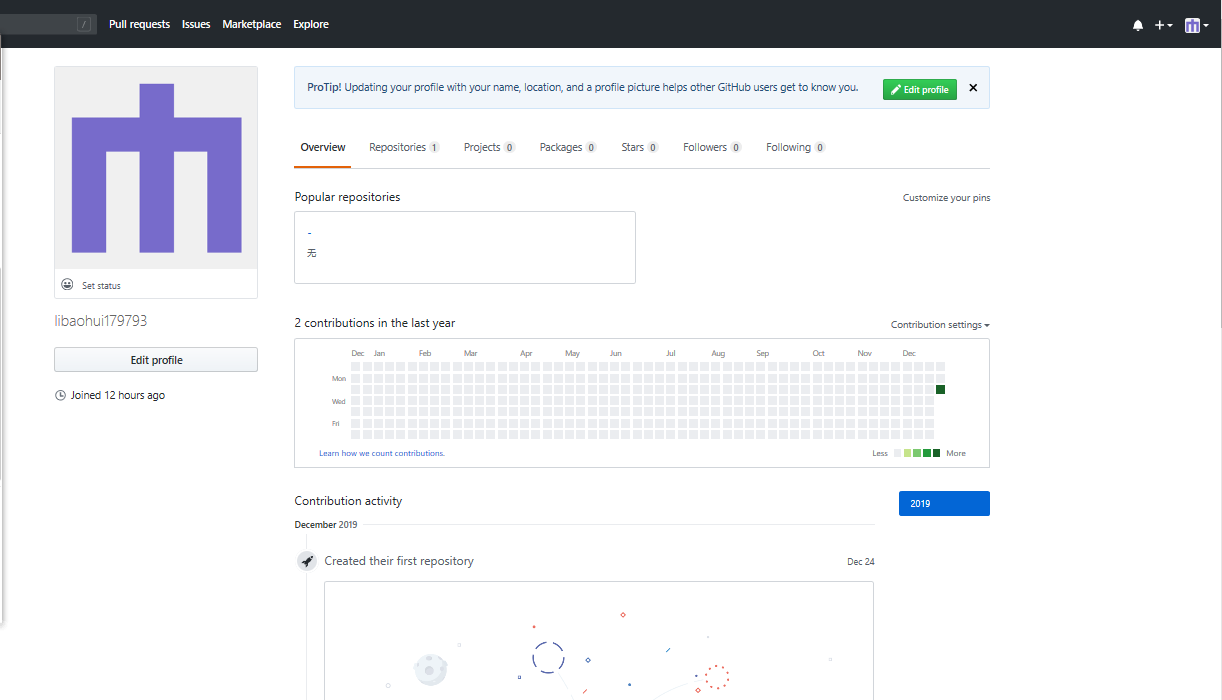
\includegraphics[scale=0.4]{Github}
\caption{Github网址:https://github.com/libaohui179793/-}
\label{fig:Github}
\end{figure}

\begin{figure}[htb!]
\item\subsection{观察者}
\centering
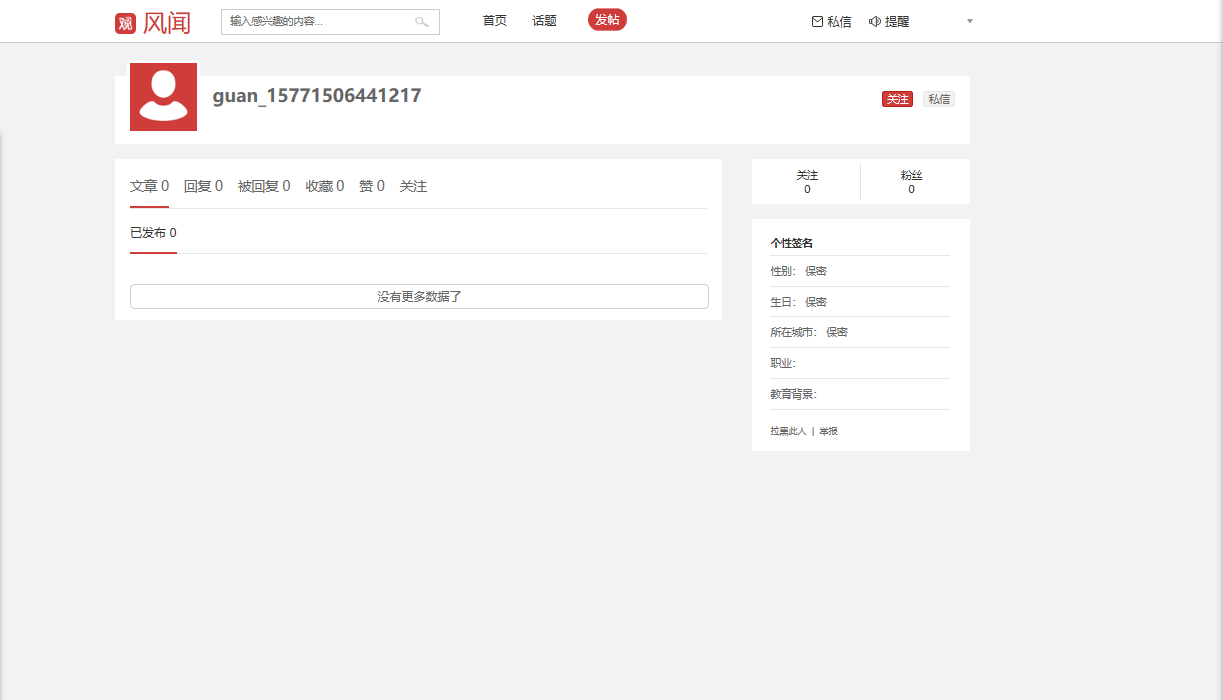
\includegraphics[scale=0.35]{guanchazhe}
\caption{观察者}
\label{fig:guanchazhe}
\end{figure}

\begin{figure}[htb!]
\item\subsection{学习强国}
\centering
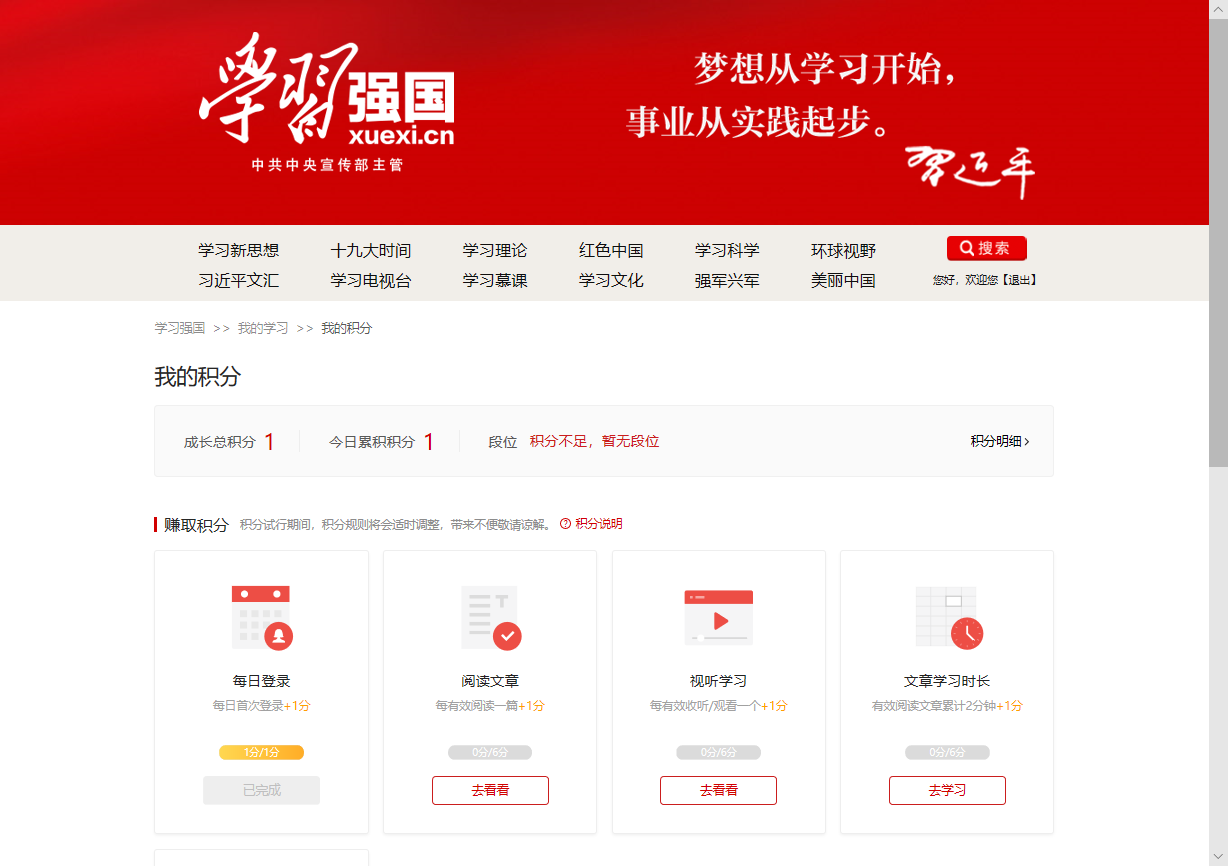
\includegraphics[scale=0.25]{xuexiqiangguo}
\caption{学习强国}
\label{fig:xuexiqiangguo}
\end{figure}

\begin{figure}[htb!]
\item\subsection{bilibili}
\centering
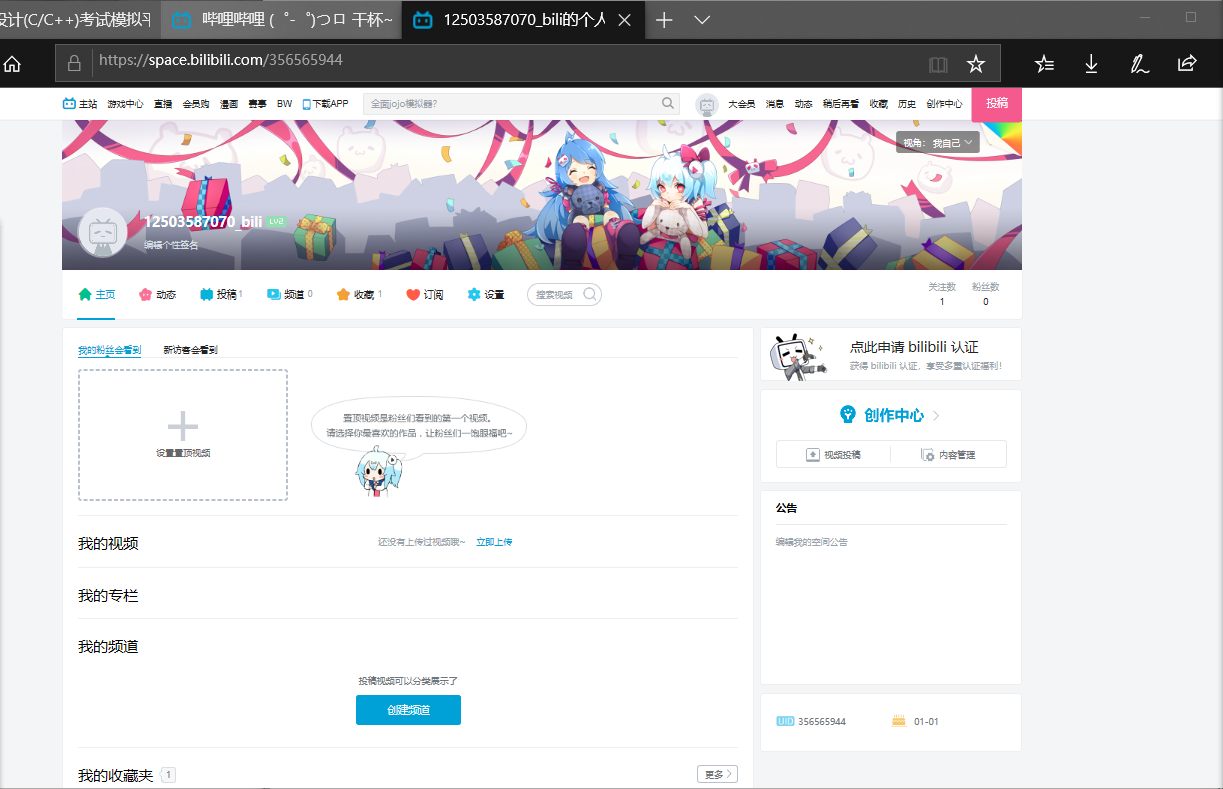
\includegraphics[scale=0.25]{bilibili}
\caption{bilibili}
\label{fig:bilibili}
\end{figure}

\begin{figure}[htb!]
\item\subsection{CSDN}
\centering
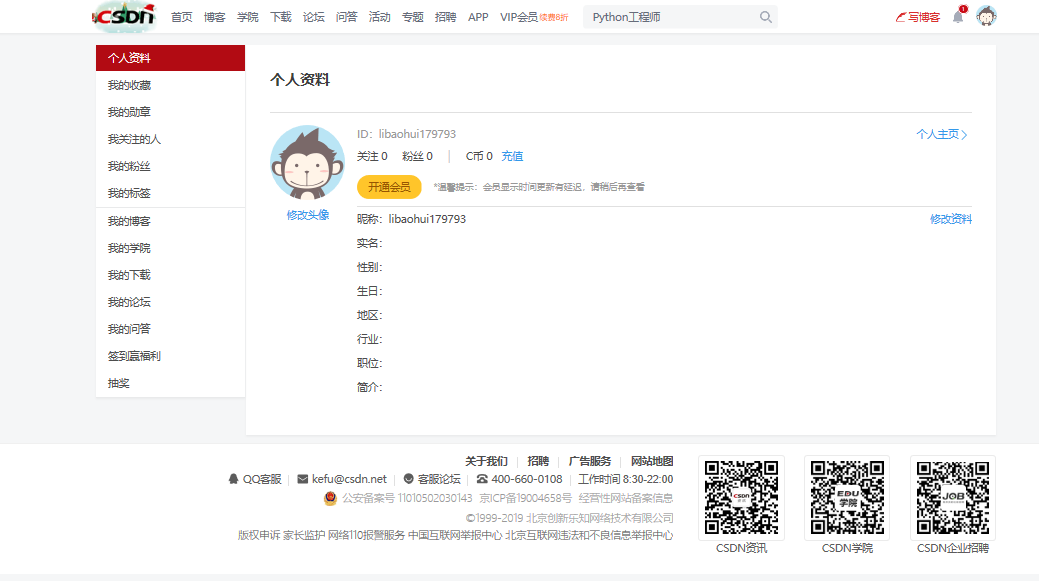
\includegraphics[scale=0.25]{CSDN}
\caption{CSDN网址:https://i.csdn.net/\#/uc/profile}
\label{fig:CSDN}
\end{figure}

\begin{figure}[htb!]
\item\subsection{博客网}
\centering
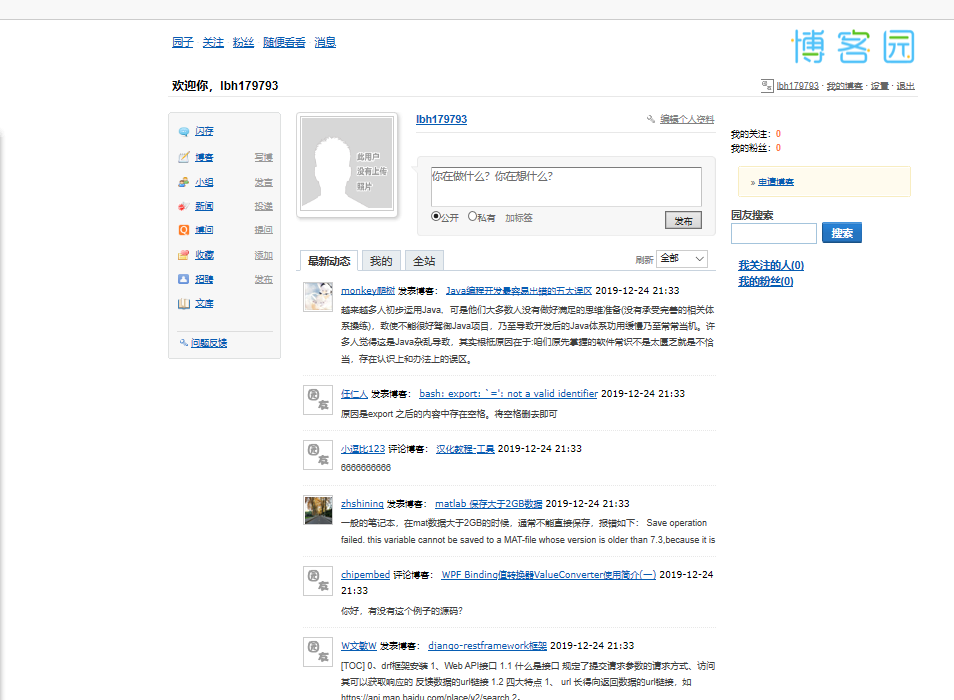
\includegraphics[scale=0.25]{bokeyuan}
\caption{博客园网址:https://home.cnblogs.com/}
\label{fig:bokeyuan}
\end{figure}

\begin{figure}[htb!]
\item\subsection{小木虫}
\centering
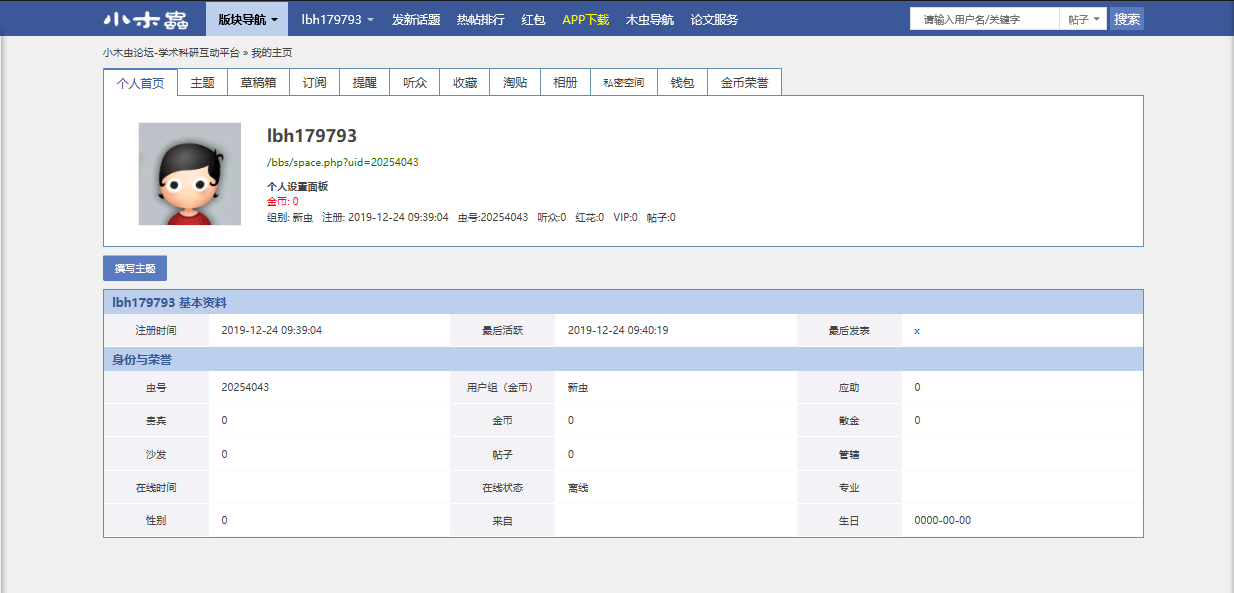
\includegraphics[scale=0.25]{xiaomuchong}
\caption{小木虫网址:http://muchong.com/bbs/space.php?uid=20254043}
\label{fig:xiaomuchong}
\end{figure}

\end{itemize}

\begin{enumerate}
    \item 电子工程师社区:工程师周亮《鸿蒙操作系统的发布将会在未来10到20年里具有里程碑意义》
    \item 百度文库:LeoGo科技《华为正式发布鸿蒙操作系统,震惊和支持之后正面看待鸿蒙优缺点!》
    \item 搜狐:《黄卫伟:华为面临的4大挑战和对策》 
    \item H. M. Hassan \& Charles Hutchinson. Natural Resource and Environmental Information for Decision Making. A World Bank Publication, Washington D. C., USA, 1995
    \item Willian K, Michener, James W. Brunt \& Susan G. Stafford. Environmental Information Management and Analysis: Ecosystem to Global Scales, Taylor \& Franics Ltd, London, Britain,1994
\end{enumerate}
\end{document}
